\chapter{Dynamical Characterization of Reservoir Responses}
\label{chap:dynamics}

\section{Introduction and Motivation}

This chapter asks what can be learned by summarizing the reservoir trajectory rather than only its final embedding. The summaries are explicitly defined functions of a driven nonlinear system. They make intermediate computations inspectable, but they are not assumed to be physiological measurements or clinically meaningful variables.

The preceding chapters specify a fixed reservoir followed by channel-organized analysis. Here the reservoir trajectory is summarized with quantities that have stated definitions, units, or scales, and their within-cohort associations with input condition are described.

The analysis uses the selected reservoir operating point ($\beta = 0.05$, $M_{th}=0.5$, $N_{res}=256$), extracts seven summaries from all $633$ SHAPE observations, and screens variation by affective condition and clinical label. The summaries cover sparse activity, trajectory complexity, and response persistence. They make the reservoir response analyzable without implying clinical actionability.

All seven dynamical metrics have nominal Friedman $p < 0.05$ for the condition comparison, but this seven-test family was not multiplicity controlled. The mean effect-size magnitude in the two-member temporal-structure group ($\hat{H}_{\pi}$, $\tau_{AC}$) is $2.4\times$ that of the four-member amplitude-associated group. None of the $49$ channel-averaged metric--diagnosis screens has nominal $p<0.05$, and the clinical balanced-accuracy estimates are near chance. The later ``excitability--persistence'' label is therefore a descriptive name for an in-sample principal component, not a patient-level scale.

\section{Notation and Formal Definitions}
\label{sec:dynamics_notation}

The following definitions specify the reservoir state and the summaries used in this chapter.

\subsection{The LSM as a Driven Dynamical System}

The selected LSM reservoir has $N_{res}=256$ leaky integrate-and-fire neurons, fixed random input weights $\mathbf{W}^{in} \in \mathbb{R}^{N_{res} \times N_f}$, fixed random recurrent weights $\mathbf{W}^{rec} \in \mathbb{R}^{N_{res} \times N_{res}}$, membrane decay parameter $\beta=0.05$ (corresponding to $\tau_m \approx 20$ time steps), and firing threshold $M_{th}=0.5$. The reservoir receives one EEG channel as its input.

\paragraph{Definition 6.1 (Input Process).}
For a given subject $s$ and trial $j$, let $\mathbf{u}^{(j)}_s(t) \in \mathbb{R}^{N_f}$ denote the preprocessed EEG input vector at discrete time step $t \in \{1,\ldots,T\}$, where $T$ is the epoch length and $N_f$ is the number of input features per time step.

\paragraph{Definition 6.2 (Reservoir State).}
The retained post-update reservoir state at time $t$ is the membrane-potential vector
\begin{equation}
\mathbf{M}(t) = [M_1(t), M_2(t), \ldots, M_{N_{res}}(t)]^{\top} \in \mathbb{R}^{N_{res}}
\end{equation}
The implementation first computes the pre-reset value
\begin{equation}
\widetilde{M}_i[t] = (1-\beta)M_i[t-1](1-S_i[t-1]) + I_{tot,i}[t]
\end{equation}
where $S_i[t-1] \in \{0,1\}$ is the spike indicator at the previous step and
\begin{equation}
I_{tot,i}[t] = \sum_{j=1}^{N_f} W^{in}_{ij}u_j(t) + \sum_{\ell=1}^{N_{res}} W^{rec}_{i\ell}S_{\ell}[t-1].
\end{equation}
A spike is emitted when $\widetilde{M}_i[t] \ge M_{th}$:
\begin{equation}
S_i[t] = \Theta(\widetilde{M}_i[t]-M_{th}),
\end{equation}
and the retained state is
\begin{equation}
M_i[t]=\max\!\left(\widetilde{M}_i[t]-S_i[t]M_{th},\,0\right),
\end{equation}
where $\Theta(\cdot)$ is the Heaviside step function. Thus a unit that spikes has its threshold subtracted on the current step and its retained contribution cleared in the next-step decay term.

\paragraph{Definition 6.3 (Spike Train Matrix).}
For a given trial, the complete spike output of the reservoir is the binary matrix
\begin{equation}
\mathbf{S} \in \{0,1\}^{N_{res}\times T}, \qquad S_{i,t}=S_i[t].
\end{equation}

\paragraph{Definition 6.4 (Global Firing Rate).}
The instantaneous population firing rate at time $t$ is
\begin{equation}
r(t)=\frac{1}{N_{res}}\sum_{i=1}^{N_{res}} S_i[t].
\end{equation}

\paragraph{Definition 6.5 (Driven System Emphasis).}
For a fixed reservoir instantiation (fixed $\mathbf{W}^{in}$ and $\mathbf{W}^{rec}$), the reservoir state trajectory $\mathbf{M}(1),\mathbf{M}(2),\ldots,\mathbf{M}(T)$ is a deterministic function of the input sequence $\mathbf{u}(1),\mathbf{u}(2),\ldots,\mathbf{u}(T)$. We denote the mapping from input sequence to state trajectory as
\begin{equation}
\mathcal{R}: \mathbb{R}^{N_f \times T} \rightarrow \mathbb{R}^{N_{res} \times T}.
\end{equation}
All dynamical metrics extracted in this chapter are properties of $\mathcal{R}(\mathbf{u})$, the driven trajectory, not of $\mathcal{R}$ in isolation.

\section{Metric I: Sparse Coding Efficiency \texorpdfstring{($\Phi$)}{(Phi)}}
\label{sec:dynamics_phi}

\subsection{Theoretical Foundation}

The efficient-coding literature motivates comparing information retained by a representation with the operations needed to compute it \cite{barlow_possible_1961,olshausen_emergence_1996}. In this software implementation, spike counts can support an operation-count estimate. They cannot establish metabolic cost, physical energy use, or pathological inefficiency. The dissertation therefore treats this metric as engineering bookkeeping rather than a biological hypothesis.

\subsection{Formal Metric Definition}

\paragraph{Definition 6.6 (Total Synaptic Operations).}
For a single trial with spike train matrix $\mathbf{S}$, the total synaptic operations count is
\begin{equation}
\mathrm{SynOps} = \sum_{t=1}^{T} \left[ \sum_{i=1}^{N_{res}} S_i[t] \cdot \left(\mathrm{fan\mbox{-}out}^{rec}_i + \mathrm{fan\mbox{-}out}^{read}_i\right) \right]
\end{equation}
where $\mathrm{fan\mbox{-}out}^{rec}_i$ is the number of nonzero outgoing recurrent connections from neuron $i$ and $\mathrm{fan\mbox{-}out}^{read}_i$ is the number of readout connections. For a fully connected readout to $N_{out}$ output neurons,
\begin{equation}
\mathrm{SynOps} = \sum_{t=1}^{T} \sum_{i=1}^{N_{res}} S_i[t] \cdot (d_i^{rec}+N_{out})
\end{equation}
where $d_i^{rec}$ is the recurrent out-degree of neuron $i$.

Under sparse random connectivity with connection probability $p_c$, the expected recurrent fan-out per neuron is $p_cN_{res}$, yielding the simplified estimator
\begin{equation}
\mathrm{SynOps} \approx N_{total\_spikes}\cdot (p_cN_{res}+N_{out})
\end{equation}
where $N_{total\_spikes}=\sum_{i,t} S_{i,t}$ is the total spike count over the epoch.

\paragraph{Definition 6.7 (Hardware-Model Energy Estimate).}
If a specified hardware platform assigns energy $E_{syn}$ to each synaptic operation, a model-based trial estimate would be
\begin{equation}
E_{trial}=\mathrm{SynOps}\cdot E_{syn}. 
\end{equation}

\paragraph{Definition 6.8 (Decoded Information Summary).}
Let $f(\mathbf{S})$ denote a feature vector extracted from the spike train and let $\hat{y}$ be an out-of-fold prediction produced from that vector. The mutual information between the observed label and the decoded label can be computed from the out-of-fold confusion matrix:
\begin{equation}
\hat{I}(y;\hat{y})=\sum_{k=1}^{K}\sum_{\hat{k}=1}^{K} p(y=k,\hat{y}=\hat{k})\log_2\!\left(\frac{p(y=k,\hat{y}=\hat{k})}{p(y=k)\,p(\hat{y}=\hat{k})}\right).
\end{equation}
Because $y\rightarrow\mathbf{S}\rightarrow f(\mathbf{S})\rightarrow\hat{y}$ is a processing chain, $I(y;\mathbf{S})\geq I(y;\hat{y})$ by the data processing inequality. This is a dataset-level decoder summary, not a per-trial estimate of the information in the spike train. It must be computed from genuinely out-of-fold predictions; accuracy alone is insufficient to determine it.

\paragraph{Definition 6.9 (Operation-Normalized Decoder Summary).}
When fold-safe out-of-fold predictions are available, an operation-normalized descriptive summary may be reported as
\begin{equation}
\Phi_{dataset} = \frac{\hat{I}(y;\hat{y})}{\overline{\mathrm{SynOps}}} \qquad \left[\frac{\mathrm{bits}}{\mathrm{mean\ trial\ synaptic\ operation}}\right]
\end{equation}
where $\overline{\mathrm{SynOps}}$ is the mean estimated operation count per trial. This ratio is one dataset-level descriptive number. It does not define a trial-level or condition-level information efficiency distribution. A physical energy quantity would additionally require hardware-specific measurements; multiplying by a literature energy-per-operation constant provides only a hardware-model estimate.
For completeness, a hardware-model normalization would be
\begin{equation}
\Phi_E = \frac{\hat{I}(y;\hat{y})}{\overline{E}_{trial}} \qquad \left[\frac{\mathrm{bits}}{\mathrm{Joule}}\right],
\end{equation}
but it is not evaluated in this dissertation because no neuromorphic hardware was profiled.

\subsection{Auxiliary Metrics}

\paragraph{Definition 6.10 (Population Sparsity).}
The lifetime sparsity of the population response is measured by the Treves--Rolls sparsity index
\begin{equation}
a = \frac{\left(\frac{1}{N_{res}}\sum_{i=1}^{N_{res}} \bar{r}_i\right)^2}{\frac{1}{N_{res}}\sum_{i=1}^{N_{res}} \bar{r}_i^2}
\end{equation}
where $\bar{r}_i=(1/T)\sum_t S_i[t]$ is the mean firing rate of neuron $i$ over the epoch.

\paragraph{Definition 6.11 (Temporal Sparsity).}
The fraction of time steps in which the population is quiescent is
\begin{equation}
a_{temp}=\frac{1}{T}\sum_{t=1}^{T} \mathbb{1}[r(t)<\epsilon].
\end{equation}
In implementation, $\epsilon$ may be chosen as $1/N_{res}$, corresponding to at most one spike per time step.

\subsection{Scope of the Efficiency Summary}
Because $\Phi_{dataset}$ is defined from a single out-of-fold confusion matrix, it is not a participant-level variable and cannot be compared between individual HC and MDD observations. The archived analysis treated a fixed decoded-information numerator divided by each trial's spike count as though it were trial-level information efficiency. That construction is not used here. EXP-6.5 therefore reports only the observed operation-count stability; no clinical information-efficiency hypothesis is tested.

\section{Metric II: Driven Trajectory Complexity \texorpdfstring{($\Lambda$)}{(Lambda)}}
\label{sec:dynamics_lambda}

\subsection{Theoretical Foundation}

The edge-of-chaos hypothesis motivates studying contraction and expansion in recurrent systems \cite{langton_computation_1990,bertschinger_real-time_2004}. For a driven reservoir, the relevant quantity is the separation rate of nearby reservoir trajectories under the \emph{same} input, not the autonomous Lyapunov spectrum. Any clinical direction proposed below is exploratory; no theorem links diagnostic status to the complexity of this fixed reservoir's response.

\subsection{Formal Metric Definitions}

\subsubsection{The Largest Lyapunov Exponent of the Driven Reservoir}

\paragraph{Definition 6.12 (Driven Lyapunov Exponent).}
Consider the driven reservoir as a discrete-time dynamical system
\begin{equation}
\mathbf{M}[t+1]=\mathbf{F}(\mathbf{M}[t],\mathbf{u}[t]).
\end{equation}
The driven Lyapunov exponent quantifies the average exponential rate of separation of infinitesimally close trajectories under the same input drive. Let $\delta \mathbf{M}[0]$ be a small perturbation to the initial state and let the perturbed trajectory evolve as
\begin{equation}
\mathbf{M}'[t+1]=\mathbf{F}(\mathbf{M}'[t],\mathbf{u}[t]).
\end{equation}
Then
\begin{equation}
\lambda_1 = \lim_{T\to\infty}\frac{1}{T}\sum_{t=0}^{T-1}\ln\frac{\lVert \delta \mathbf{M}[t+1]\rVert}{\lVert \delta \mathbf{M}[t]\rVert}
\end{equation}
where $\delta \mathbf{M}[t]=\mathbf{M}'[t]-\mathbf{M}[t]$.

The threshold-and-reset operation in leaky integrate-and-fire dynamics introduces a discontinuity, so the tangent-space calculation must account for spike events explicitly. Event-based Lyapunov calculations for LIF networks have been developed in prior work on spiking-network stability and can be used to motivate the projection treatment at threshold crossings \cite{monteforte_dynamic_2012}. For finite EEG epochs, the practical estimate used in this chapter follows the standard renormalization strategy associated with Benettin-style Lyapunov computation \cite{benettin_lyapunov_1980}:
\begin{enumerate}
    \item Initialize the reservoir at state $\mathbf{M}[0]$ and a nearby state $\mathbf{M}'[0]=\mathbf{M}[0]+\delta_0\hat{\mathbf{e}}$, where $\hat{\mathbf{e}}$ is a random unit vector and $\delta_0=10^{-8}$.
    \item Evolve both trajectories under the same input $\mathbf{u}(t)$ for $T_{renorm}$ steps.
    \item Compute the stretching factor $\gamma_k = \lVert \mathbf{M}'[kT_{renorm}] - \mathbf{M}[kT_{renorm}] \rVert/\delta_0$.
    \item Renormalize the perturbed trajectory along the instantaneous separation direction.
    \item Repeat for $K$ renormalization intervals and estimate
    \begin{equation}
    \hat{\lambda}_1 = \frac{1}{KT_{renorm}}\sum_{k=1}^{K}\ln(\gamma_k).
    \end{equation}
\end{enumerate}

\subsubsection{Lempel--Ziv Complexity ($C_{LZ}$)}

\paragraph{Definition 6.13 (Lempel--Ziv Complexity of Reservoir Spike Output).}
For a single neuron $i$, let $s_i=S_i[1]S_i[2]\cdots S_i[T]$ be the binary spike sequence. The normalized Lempel--Ziv complexity is
\begin{equation}
C_{LZ,i}=\frac{c(s_i)}{T/\log_2(T)}
\end{equation}
where $c(s_i)$ is the number of distinct substrings generated by the LZ76 parsing procedure. The population-level complexity is
\begin{equation}
C_{LZ}=\frac{1}{N_{res}}\sum_{i=1}^{N_{res}} C_{LZ,i}.
\end{equation}

\subsubsection{Permutation Entropy ($H_{\pi}$)}

\paragraph{Definition 6.14 (Permutation Entropy of Membrane Potential Trajectory).}
As a complementary complexity measure operating on the continuous-valued membrane potentials rather than the binary spike trains, define the global mean membrane potential
\begin{equation}
\bar{M}(t)=\frac{1}{N_{res}}\sum_{i=1}^{N_{res}} M_i[t].
\end{equation}
For embedding dimension $d$ and delay $\tau$, ordinal patterns are constructed from $[\bar{M}(t),\bar{M}(t+\tau),\ldots,\bar{M}(t+(d-1)\tau)]$. The permutation entropy is then
\begin{equation}
H_{\pi}=-\sum_{\pi\in S_d} p(\pi)\log_2 p(\pi)
\end{equation}
with normalized form
\begin{equation}
\hat{H}_{\pi}=\frac{H_{\pi}}{\log_2(d!)}.
\end{equation}
Permutation entropy was introduced by Bandt and Pompe as a natural complexity measure for time series \cite{bandt_permutation_2002}.

\subsection{Phase-Space Visualization}

\paragraph{Definition 6.15 (Reconstructed Phase Portrait).}
For visualization of a finite driven trajectory, let $\mathbf{M} \in \mathbb{R}^{N_{res}\times T}$ be the membrane-potential matrix for a given observation. Compute the PCA projection
\begin{equation}
\mathbf{z}(t)=\mathbf{W}_{PC}^{\top}(\mathbf{M}(t)-\bar{\mathbf{M}}) \in \mathbb{R}^{2}
\end{equation}
where $\mathbf{W}_{PC}=[\mathbf{w}_1,\mathbf{w}_2]$ contains the first two principal-component directions and $\bar{\mathbf{M}}$ is the temporal mean.

\subsection{Hypothesis H2}
An exploratory directional hypothesis is that reservoir trajectories driven by EEG from the complete-case control group will have larger complexity summaries than trajectories from participants with MDD:
\begin{equation}
\mathbb{E}[\Lambda\mid \mathrm{HC}] > \mathbb{E}[\Lambda\mid \mathrm{MDD}]
\end{equation}
where $\Lambda \in \{\lambda_1,C_{LZ},\hat{H}_{\pi}\}$. This hypothesis is tested in Section~\ref{sec:ch6_results}, EXP-6.6.

\section{Metric III: Relaxation Time Constant \texorpdfstring{($T$)}{(T)}}
\label{sec:dynamics_tau}

\subsection{Theoretical Foundation}

Critical slowing down describes slower recovery near some dynamical transitions \cite{scheffer_early-warning_2009}, and elevated temporal autocorrelation has been proposed as an early-warning signal in affective time series \cite{vandeleemput_critical_2014,wichers_critical_2016}. The present quantity is narrower: it summarizes decay in the fixed reservoir's population response over an observed epoch. It is not a cortical recovery or tipping-point estimate.

\subsection{Formal Metric Definitions}

\subsubsection{Exponential Relaxation Time ($\tau_{relax}$)}

\paragraph{Definition 6.16 (Relaxation Time Constant).}
Consider the global firing rate $r(t)$ during the post-stimulus window $[t_{onset},t_{end}]$. Define
\begin{equation}
r_{peak}=\max_{t\in[t_{onset},t_{end}]} r(t), \qquad t_{peak}=\arg\max_{t\in[t_{onset},t_{end}]} r(t).
\end{equation}
The relaxation phase is $[t_{peak},t_{end}]$. Model the decay of the firing-rate envelope as
\begin{equation}
r(t) \approx r_{\infty} + (r_{peak}-r_{\infty})\exp\left(-\frac{t-t_{peak}}{\tau_{relax}}\right), \qquad t\ge t_{peak}
\end{equation}
where $r_{\infty}$ is estimated from the final portion of the epoch.

\subsubsection{Autocorrelation Decay Rate}

\paragraph{Definition 6.17 (Lag-$k$ Autocorrelation of Population Firing Rate).}
The normalized autocorrelation function of the global firing rate is
\begin{equation}
\rho(k)=\frac{\sum_{t=1}^{T-k}(r(t)-\bar{r})(r(t+k)-\bar{r})}{\sum_{t=1}^{T}(r(t)-\bar{r})^2}
\end{equation}
where $\bar{r}=(1/T)\sum_t r(t)$.

\paragraph{Definition 6.18 (Autocorrelation Decay Constant).}
Define
\begin{equation}
\tau_{AC}=\min\{k\ge 1: \rho(k)\le e^{-1}\}
\end{equation}
or estimate $\tau_{AC}$ by fitting an exponential decay model to $\rho(k)$.

\subsubsection{Attractor Depth via Return-to-Baseline Time}

\paragraph{Definition 6.19 (Return-to-Baseline Time).}
Let the baseline firing rate be
\begin{equation}
r_{baseline}=\frac{1}{|[1,t_{onset}]|}\sum_{t=1}^{t_{onset}} r(t).
\end{equation}
The return-to-baseline time is
\begin{equation}
T_{RTB}=\min\left\{t>t_{peak}: r(t')\le r_{baseline}+\alpha(r_{peak}-r_{baseline})\ \forall\ t'\in[t,t+\Delta]\right\}-t_{peak}
\end{equation}
where $\alpha\in(0,1)$ is a threshold fraction and $\Delta$ is a sustain window.

\subsection{Linearized Decay Analogy}

For an autonomous system linearized near a stable operating point, the eigenvalue of largest magnitude inside the unit disk determines the slowest decay mode. If that eigenvalue is $\mu_{max}$, then
\begin{equation}
\tau_{relax}^{(slow)} = -\frac{1}{\ln|\mu_{max}|}.
\end{equation}
As $|\mu_{max}|\rightarrow 1^{-}$, this linearized time constant increases. The driven, thresholded reservoir analyzed here does not meet this simple model exactly, so the equation is contextual rather than an identification of an energy landscape or critical point.

\subsection{Hypothesis H3}
As an exploratory engineering hypothesis, EEG from participants with MDD may place the fixed reservoir in a regime with a longer measured relaxation time than EEG from healthy controls:
\begin{equation}
\mathbb{E}[\tau_{relax}\mid \mathrm{MDD}] > \mathbb{E}[\tau_{relax}\mid \mathrm{HC}].
\end{equation}
This hypothesis is tested in Section~\ref{sec:ch6_results}, EXP-6.6. The test concerns the response of the fixed reservoir to the observed EEG; it is not a test of cortical criticality and does not estimate a cortical relaxation time.

\section{Validity and Scope of Reservoir-Derived Measures}
\label{sec:dynamics_fidelity}

This section states the conditions under which a quantity extracted from the driven reservoir can be interpreted. The analysis distinguishes three objects: the latent cortical process, the scalp EEG observation, and the response of the fixed reservoir to that observation. The metrics in this chapter describe the third object. They are not estimators of latent cortical invariants unless a separate validation establishes such a relationship.

\subsection{Fixed-Transformation Perspective}

A fixed transformation can be characterized by how it responds to controlled and observed inputs. The reservoir is treated in that limited sense: as a specified nonlinear operator whose internal state is available for inspection. It was not calibrated as a scientific instrument. The metrics are functionals of the \emph{driven reservoir response}, not latent cortical invariants.

In particular, the reservoir relaxation time is not the relaxation time of the cortex. It is a response functional of a specified nonlinear filter. Reliability across repeated recordings, reservoir initializations, and preprocessing choices would be required before that functional could support an individual-level interpretation.

\subsection{Formal Signal-Chain Setup}

Let $\theta \in \Theta$ denote a latent clinical or affective state parameter, let $\mathbf{X}(t;\theta)$ denote the latent cortical source process, and let the observed EEG be modeled as
\begin{equation}
\mathbf{u}(t;\theta)=\mathbf{L}\mathbf{X}(t;\theta)+\boldsymbol{\eta}(t)
\end{equation}
where $\mathbf{L}$ is a lead-field or mixing operator and $\boldsymbol{\eta}(t)$ denotes sensor noise. Let $\mathbf{M}(t;\theta,\omega)$ denote the reservoir membrane-potential trajectory produced by input $\mathbf{u}(t;\theta)$ under reservoir instantiation $\omega=(\mathbf{W}^{in},\mathbf{W}^{rec})$, and let $\Psi[\mathbf{M}]$ denote a dynamical functional such as $\Phi$, $\lambda_1$, or $\tau_{relax}$.

The full processing chain can then be written as
\begin{equation}
\theta \rightarrow \mathbf{X}(t;\theta) \rightarrow \mathbf{u}(t;\theta) \rightarrow \mathbf{M}(t;\theta,\omega) \rightarrow \Psi(\theta,\omega).
\end{equation}
The three core validity questions are then:
\begin{enumerate}
    \item Is $\mathbf{M}(t;\theta,\omega)$ effectively determined by $\mathbf{u}(t;\theta)$ rather than by its initial condition?
    \item Does the reservoir retain sufficient information about the clinically relevant structure in $\mathbf{u}(t;\theta)$?
    \item Does the chosen functional $\Psi$ preserve the ordering or magnitude of the input property of interest?
\end{enumerate}
These questions separate state reproducibility, retained task information, and external validity. Satisfying one does not imply the others.

\subsection{Input Determinism: Echo State Property and Generalized Synchronization}

To interpret the reservoir as an input-determined filter, its dependence on the initial state must decay for the input class under study. The echo state property formalizes such loss of initial-condition dependence. Simple spectral-radius heuristics are insufficient even for smooth tanh reservoirs, and the property belongs to the driven system rather than to the recurrent matrix alone \cite{yildiz_re-visiting_2012}. The piecewise-smooth LIF update requires at least the same caution.

Formally, the reservoir satisfies the ESP with respect to an input class $\mathcal{U}$ if, for every bounded input sequence $\mathbf{u}\in\mathcal{U}$ and every pair of initial conditions $\mathbf{M}_0,\mathbf{M}_0'$,
\begin{equation}
\lim_{t\rightarrow\infty}\left\|\mathbf{M}(t;\mathbf{M}_0,\mathbf{u})-\mathbf{M}(t;\mathbf{M}_0',\mathbf{u})\right\|=0.
\end{equation}
A fully rigorous sufficient condition for the particular discretized LIF reservoir used here is nontrivial because the threshold-and-reset mechanism breaks global smoothness. For that reason, the strongest defensible statement is not a universal theorem for all bounded inputs, but an input-class statement: if the driven reservoir has negative conditional Lyapunov exponent over the input family of interest, then it contracts initial-condition differences and behaves as an input-determined filter. That logic is entirely consistent with generalized synchronization theory, which states that a driven system can converge onto a synchronization manifold that is a deterministic function of the input history \cite{rulkov_generalized_1995,yildiz_re-visiting_2012}.

Accordingly, a negative driven conditional Lyapunov estimate is used here as evidence of contraction for the tested input family:
\begin{equation}
\lambda_1^{(driven)} < 0 \quad \Longrightarrow \quad \mathbf{M}(t) \approx \psi(\mathbf{u}(t),\mathbf{u}(t-1),\ldots)
\end{equation}
after transient decay, for the specific operating regime under study. This empirical criterion does not prove a global echo-state property for all bounded inputs and does not by itself prove separation between stimulus classes.

\subsection{Fading Memory and Effective Memory Horizon}

Once the state is a function of the input history, one still needs a practical bound on how much history matters. Reservoir systems with the fading-memory property weight remote lags less strongly than recent lags. An effective memory horizon $T_{mem}$ can therefore be defined operationally as the lag beyond which a controlled perturbation has negligible measured effect. The heuristic $T_{mem}\approx -1/\lambda_1$ may be useful near a uniformly contracting linearization, but it is not an identity for a thresholded, input-driven reservoir and is not used as a measured cortical timescale.

\subsection{Information-Theoretic Bounds}

The processing chain $\theta \rightarrow \mathbf{u} \rightarrow \mathbf{M} \rightarrow \Psi$ is a Markov chain. Therefore the data processing inequality implies
\begin{equation}
I(\theta;\Psi)\leq I(\theta;\mathbf{M})\leq I(\theta;\mathbf{u}),
\end{equation}
so neither the reservoir nor the downstream functional can create new information about the latent state that was not already present in the EEG input \cite{cover_elements_2006}. This bound is a necessary guardrail on the interpretation of Chapter 4 results. When the reservoir increases the Fisher Discriminant Ratio or improves downstream classification accuracy, the correct reading is that it improves \emph{representation geometry for the chosen decoder}, not that it increases mutual information in violation of DPI.

Any reservoir-derived metric must therefore be evaluated relative to information already present in the observed EEG, not relative to an unobserved cortical state.

\subsection{Takens-Type Embedding and Dynamical Sufficiency}

Takens' original theorem concerns smooth, deterministic, autonomous dynamical systems observed through generic scalar functions; under those assumptions, a delay embedding can reconstruct the attractor up to a diffeomorphism \cite{takens_detecting_1981}. Those assumptions do \emph{not} hold literally for noisy, volume-conducted EEG, and they certainly do not hold automatically for a discontinuous spiking reservoir. Any appeal to Takens in this dissertation must therefore be treated as an analogy supported by more recent reservoir-embedding results, not as a direct theorem about the SHAPE EEG itself.

Recent ESN theory is relevant but does not close this gap. Hart, Hook, and Dawes show that a suitable ESN trained on observations of an invertible dynamical system can induce an echo-state map that is generically an embedding with positive probability \cite{hart_embedding_2020}. Grigoryeva and Ortega establish fading-memory and approximation properties for reservoir systems under bounded inputs \cite{grigoryeva_echo_2018}. Those assumptions do not prove that the LIF reservoir used here is a diffeomorphic embedding of latent cortical dynamics. The results motivate a representation hypothesis; they are not presented as a theorem about SHAPE EEG.

\subsection{Metric-Specific Validity and Monotonicity}

The most difficult issue is not state reconstruction; it is whether a chosen functional of the reservoir trajectory preserves the ordering of the corresponding input property.

\paragraph{Complexity metrics.}
For symbolic measures such as Lempel--Ziv complexity and permutation entropy, no general monotonic mapping from input complexity to reservoir-output complexity is assumed. A nonlinear filter can increase or decrease either measure. Direct comparison with input-domain measures and controlled surrogates is therefore necessary \cite{lempel_complexity_1976,bandt_permutation_2002,zunino_permutation_2017,little_permutation_2016}.

\paragraph{Driven Lyapunov exponent.}
The driven Lyapunov exponent is a joint property of the input--reservoir system, not an estimator of the cortical Lyapunov spectrum. It depends on the reservoir Jacobian along the driven trajectory and on how the input positions neurons relative to threshold. It is therefore reported only as a reservoir-stability descriptor.

\paragraph{Relaxation-time metrics.}
During a locally linear decay phase, the population-rate time constant can depend on both intrinsic reservoir contraction and the autocorrelation structure of the input. It is therefore an input-mediated effective reservoir time constant. Its physiological meaning is not established here.

\subsection{Empirical Validation Requirements}

The theoretical considerations above are not substitutes for empirical validation. A complete validation would include:
\begin{enumerate}
    \item \textbf{Echo-state verification:} initialize the same reservoir/input pair from widely separated initial conditions and verify exponential convergence of the state difference.
    \item \textbf{Cross-initialization reliability:} compute ICC$(3,1)$ for each dynamical metric across multiple reservoir initializations and require at least good reliability.
    \item \textbf{Surrogate testing:} compare real-input metrics against phase-randomized or otherwise structure-destroyed surrogates. This must be interpreted carefully because IAAFT-type surrogates can themselves exhibit residual Fourier-phase issues if used incautiously \cite{rath_revisiting_2012}.
    \item \textbf{Direct raw-EEG correlation:} correlate reservoir metrics with directly measured EEG complexity or autocorrelation statistics to demonstrate grounding in the input process.
    \item \textbf{Permutation-based group inference:} use label-permutation tests to avoid overreliance on fragile parametric assumptions in small clinical cohorts.
\end{enumerate}

\subsection{Interpretive Boundary}

The driven reservoir must forget initial conditions over the tested input family; separability claims must be phrased as changes in decoder-accessible geometry rather than creation of information; and each proposed descriptor requires reliability, surrogate, and input-domain validation. The experiments below satisfy only part of that program. The resulting quantities are therefore treated as descriptive engineering measures of the reservoir response, not as biomarkers or direct physiological measurements.

\section{Experimental Protocol}
\label{sec:dynamics_protocol}

All experiments use the $211$-subject, three-class SHAPE dataset and preprocessing pipeline established in Chapter~\ref{chap:arspi_net}. For each of $633$ observations ($211$ subjects $\times$ $3$ conditions), $34$ EEG channels are individually processed through the fixed reservoir ($N_{res} = 256$, $\beta = 0.05$, $M_{th}=0.5$), producing $21{,}522$ total reservoir runs. The seven primary summaries are total spikes, mean firing rate, rate entropy, rate variance, temporal sparsity, permutation entropy, and autocorrelation decay. Four auxiliary summaries are also retained for sensitivity analyses. Theta-band ($4$--$8$ Hz) phase-concentration matrices are computed from the full-resolution $1{,}024$~Hz EEG for Chapter~\ref{chap:synthesis}. Statistical analysis uses within-subject paired comparisons for condition effects and between-group comparisons for clinical effects. Unless a correction is explicitly stated, the reported $p$ values are exploratory nominal values rather than family-wise confirmatory tests. Raw observations are presented in Appendix~\ref{app:ch6_figs}.


\section{Experimental Results}
\label{sec:ch6_results}

\subsection{EXP-6.1: Exploratory Condition Associations Across Seven Metrics}

All seven primary metrics have nominal Friedman $p<0.05$ (Figure~\ref{fig:ch6_condition_effects}). Negative and Pleasant have similar profiles, while Neutral is the largest contrast. The archived pairwise tests report nominal differences for Negative--Neutral and Neutral--Pleasant across all seven metrics and no nominal Negative--Pleasant difference. The largest standardized contrast is observed for $\tau_{AC}$: Negative ($5.65$) $>$ Pleasant ($5.50$) $>$ Neutral ($4.92$; $d_z=+0.35$ for Negative--Neutral). Because the seven omnibus tests and their post-hoc contrasts form a multiple-testing family, these results are treated as exploratory until reproduced under a prespecified correction.

\begin{figure}[H]
    \centering
    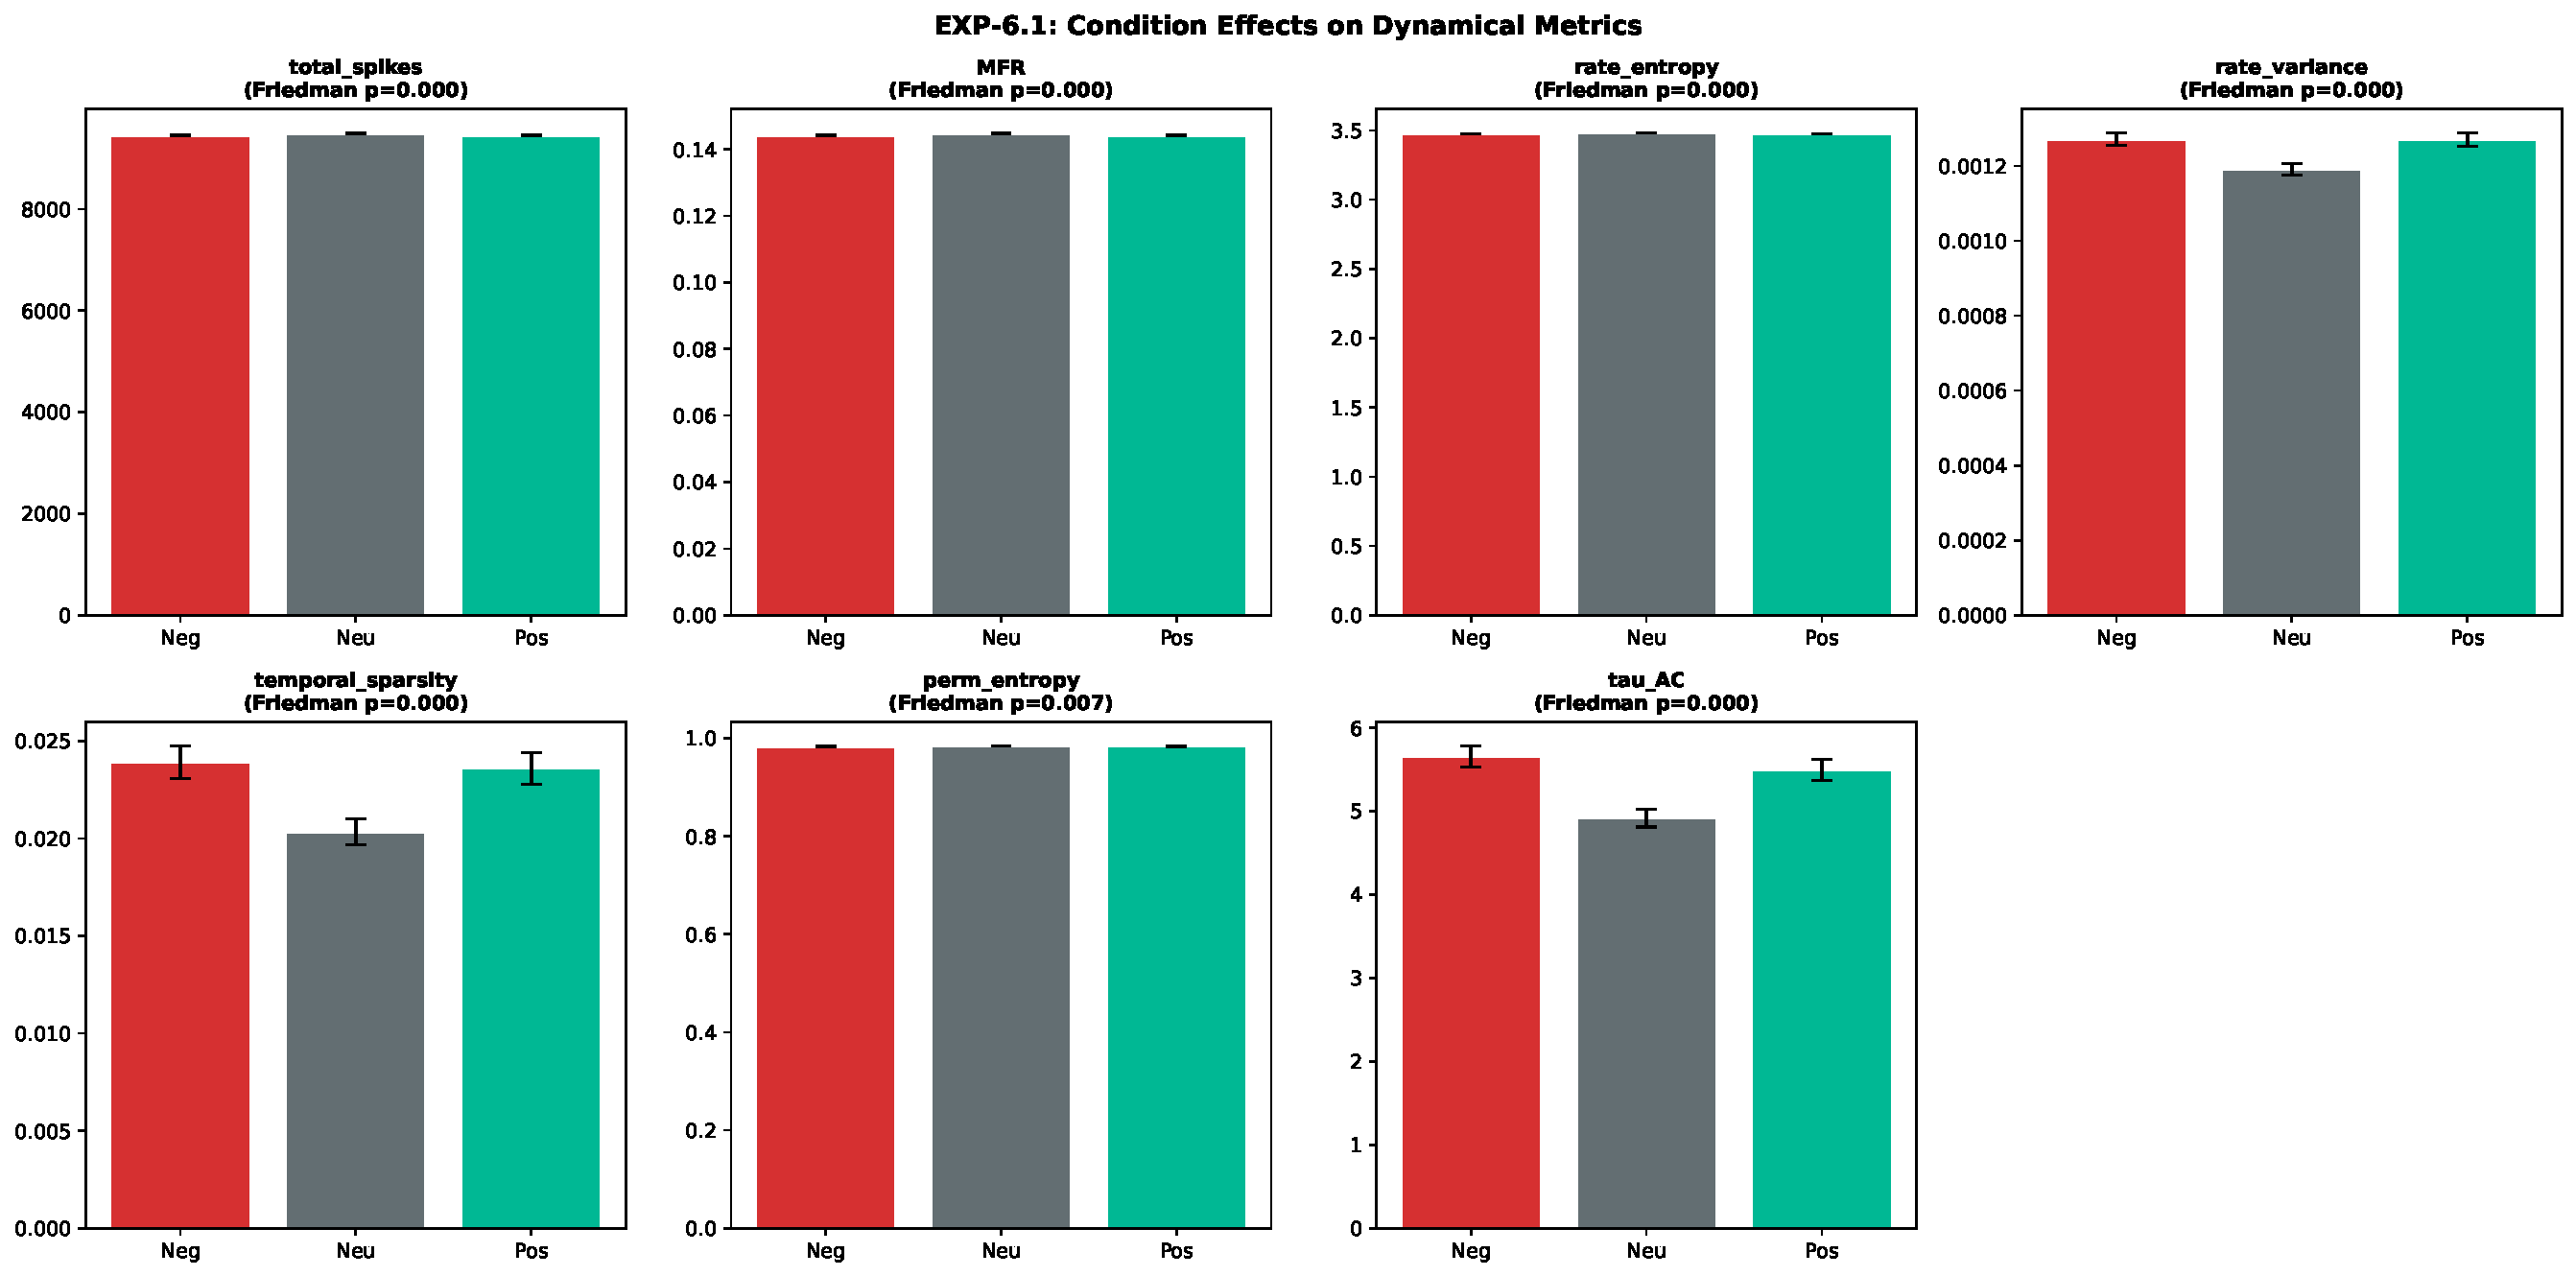
\includegraphics[width=\textwidth]{pictures/chDynamics/fig01_condition_effects.pdf}
    \caption{Exploratory condition comparisons for seven primary dynamical metrics ($N = 211$ participants, Friedman tests). All seven omnibus tests have nominal $p<0.05$. The displayed Negative and Pleasant means are close, while contrasts involving Neutral are larger. The family was not evaluated as a prespecified confirmatory test.}
    \label{fig:ch6_condition_effects}
\end{figure}

\subsection{EXP-6.2: Descriptive Metric-Family Effect-Size Ratio}

For the small Negative--Pleasant contrasts, the mean absolute effect in the two-member temporal-structure family ($\hat{H}_{\pi}$ and $\tau_{AC}$; mean $|d_z|=0.058$) is $2.4$ times the mean in the four-member amplitude-tracking family (mean $|d_z|=0.024$; Figure~\ref{fig:ch6_metric_families}). This is a descriptive ratio of two small, differently sized metric families; it is not a direct inferential test that temporal organization is uniquely responsible for condition encoding.

\begin{figure}[H]
    \centering
    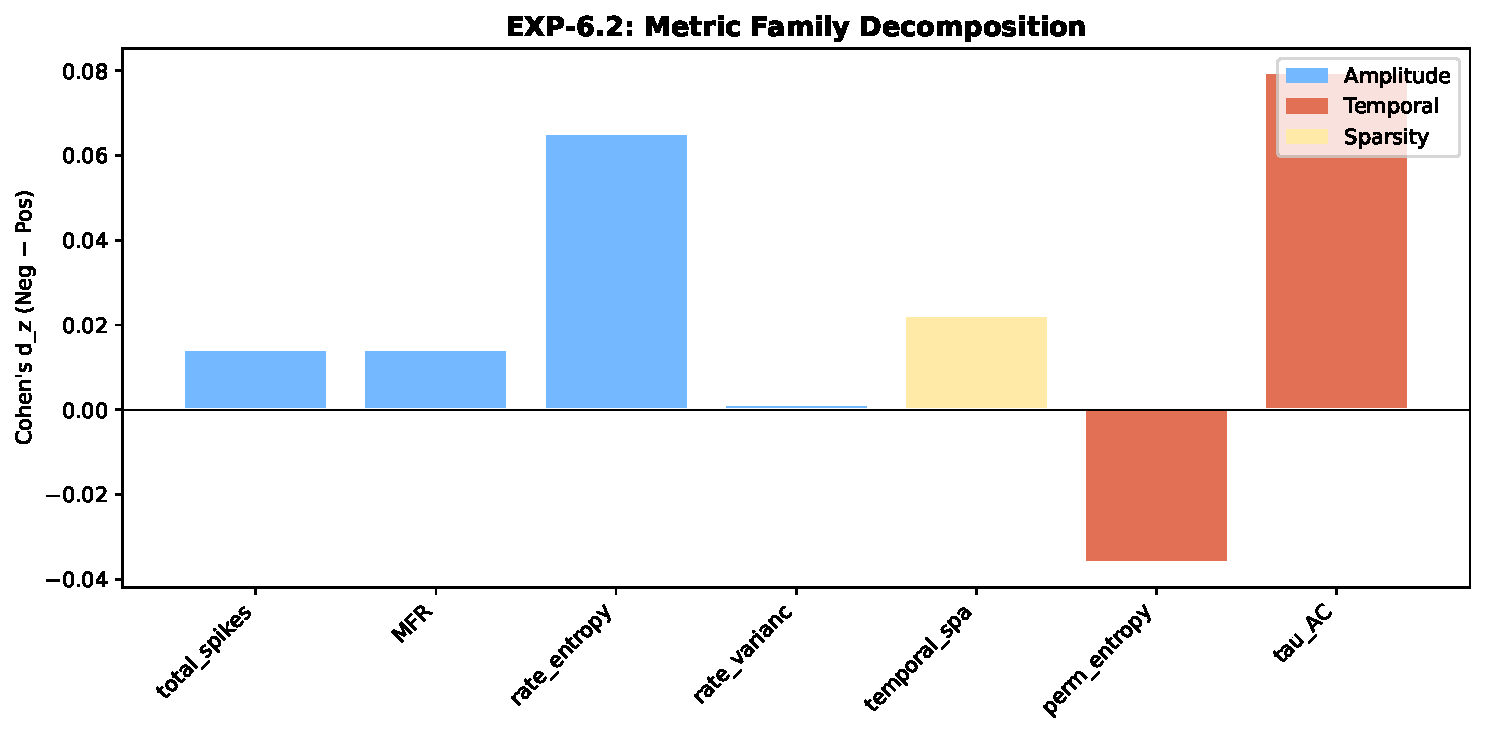
\includegraphics[width=0.85\textwidth]{pictures/chDynamics/fig02_metric_families.pdf}
    \caption{Descriptive metric-family comparison for Negative--Pleasant paired effect sizes ($d_z$). The two temporal-structure metrics have a mean absolute effect $2.4$ times that of the four amplitude-tracking metrics, but all effects in this comparison are small and the family contrast was not directly tested.}
    \label{fig:ch6_metric_families}
\end{figure}

\subsection{EXP-6.3: No Detected Clinical Group Differences}

None of the $49$ metric--group comparisons ($7$ metrics $\times$ $7$ clinical variables) has nominal $p<0.05$ (Figure~\ref{fig:ch6_clinical_heatmap}). The largest observed difference is MDD on $\tau_{AC}$: $5.44$ for MDD versus $5.19$ for non-MDD ($\Delta=+0.24$). These tests provide no evidence of group differences at the sensitivity of this sample; they do not establish equality or absence of smaller effects.

\begin{figure}[H]
    \centering
    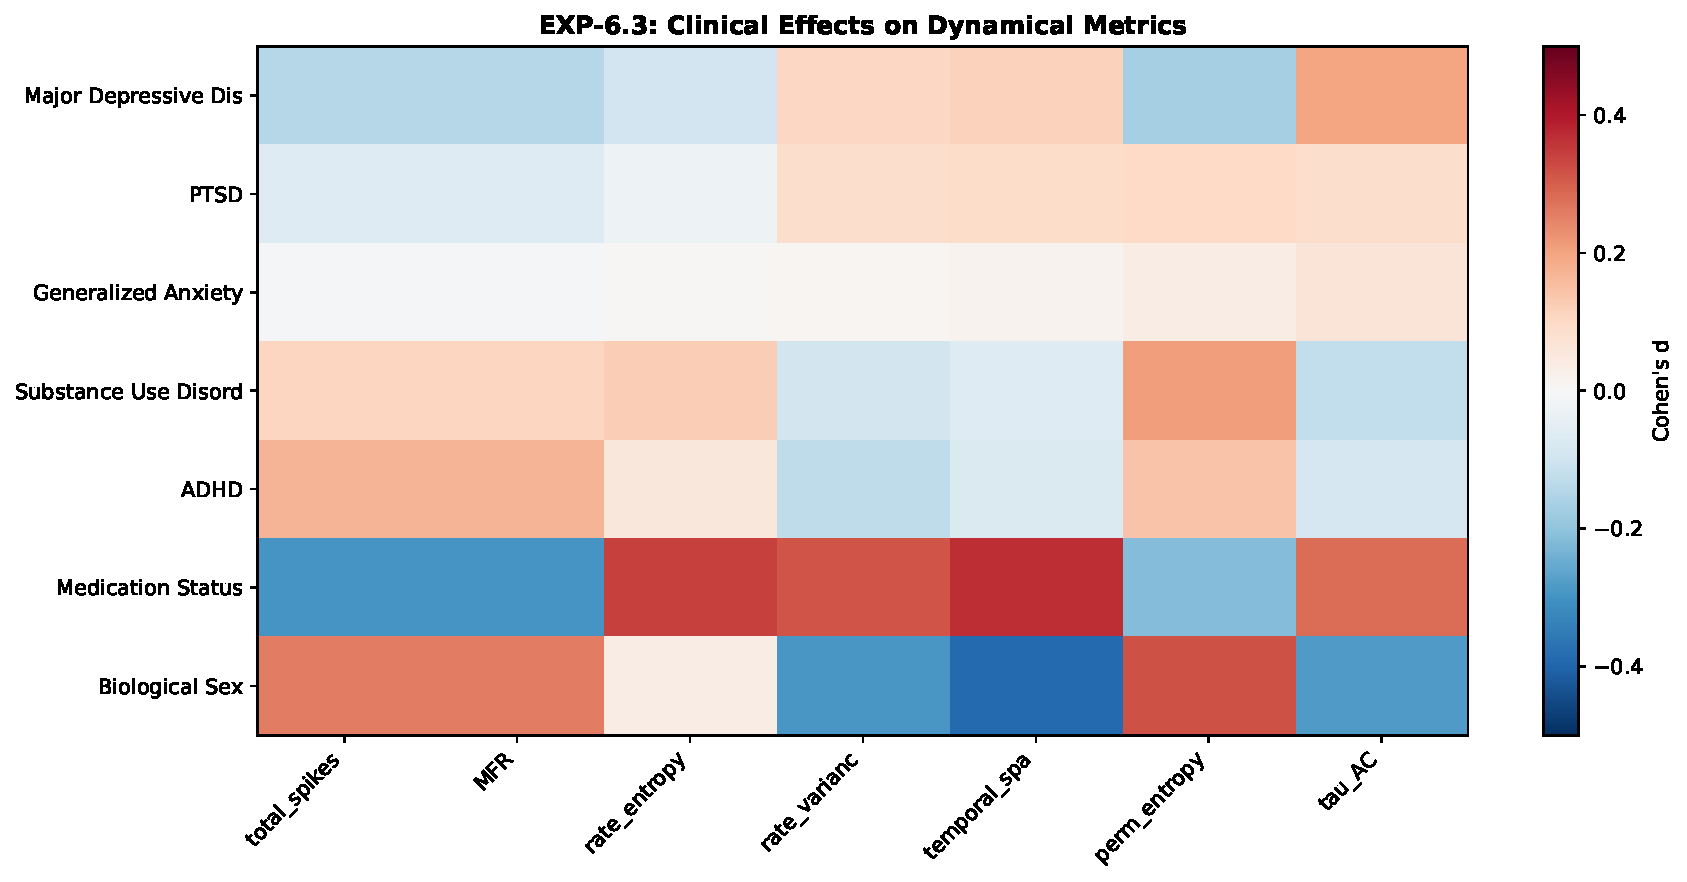
\includegraphics[width=\textwidth]{pictures/chDynamics/fig03_clinical_heatmap.pdf}
    \caption{Exploratory transdiagnostic comparisons for seven dynamical metrics and seven grouping variables. None of the $49$ nominal tests has $p<0.05$. The result is a lack of detected group differences, not evidence that clinical effects are absent.}
    \label{fig:ch6_clinical_heatmap}
\end{figure}

The condition contrasts are larger than the observed channel-averaged clinical contrasts in this cohort. That difference is descriptive: it does not show that the reservoir distinguishes stimuli but not people, and it cannot be compared directly with the broad, partly uncorrected graph search in Chapter~\ref{chap:arspi_net}.

\subsection{EXP-6.4: No Significant Condition \texorpdfstring{$\times$}{by} Clinical Interactions}

Zero of $35$ interaction tests ($7$ metrics $\times$ $5$ clinical variables) has nominal $p<0.05$ (Figure~\ref{fig:ch6_interactions}). The archived sample means for MDD and non-MDD $\tau_{AC}$ reactivity are $+0.24$ and $-0.01$, respectively. Without a supported interaction, that direction is descriptive and does not confirm the hypothesis.

\begin{figure}[H]
    \centering
    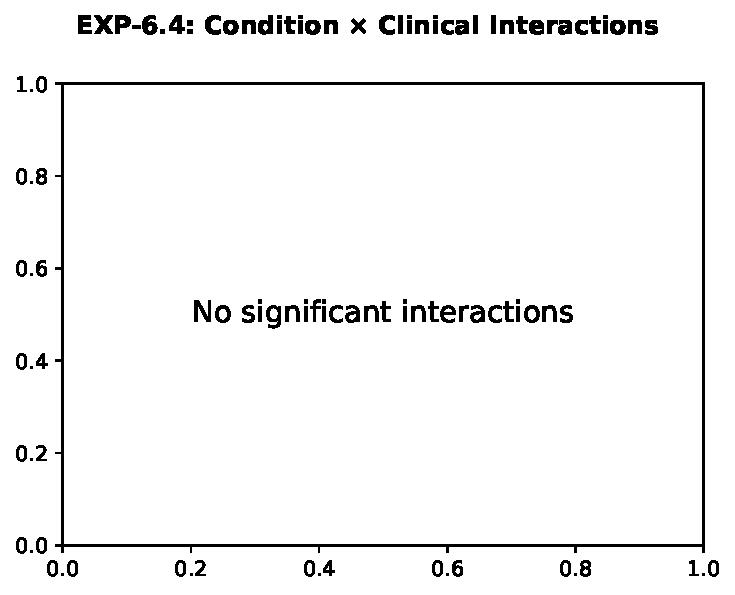
\includegraphics[width=0.85\textwidth]{pictures/chDynamics/fig04_interactions.pdf}
    \caption{Exploratory condition-by-group screens using Negative--Pleasant reactivity. None of the 35 nominal interaction tests has $p<0.05$; displayed directions do not confirm the proposed clinical hypotheses.}
    \label{fig:ch6_interactions}
\end{figure}

\subsection{EXP-6.5: Estimated Operation Counts Are Stable Across Conditions}

The archived analysis shows that total spike count, and therefore the estimated synaptic-operation denominator, varies by approximately $0.5\%$ across conditions at the selected operating point. The earlier trial-level ``bits/spike'' construction used one accuracy-derived numerator for every observation and is not a valid per-trial mutual-information estimate; it is omitted. A fold-safe decoded-information summary would require new out-of-fold predictions after the preprocessing corrections described in Chapter~\ref{chap:arspi_net}. This experiment therefore supports only the narrower observation that gross firing cost is stable across conditions.

\subsection{EXP-6.6: HC vs MDD Hypothesis Tests}

All archived directional comparisons have $p>0.3$ (Figure~\ref{fig:ch6_hc_vs_mdd}). The archived ``HC'' group contains 27 records because five participants with incomplete diagnostic panels were treated as negative; only 22 complete cases are negative for all five primary diagnoses. The resulting HC--MDD contrasts are therefore not valid complete-case control comparisons and are retained only to document the prior analysis. No participant-level $\Phi$ comparison is reported because the operation-normalized decoder summary is defined at the dataset level.

\begin{figure}[H]
    \centering
    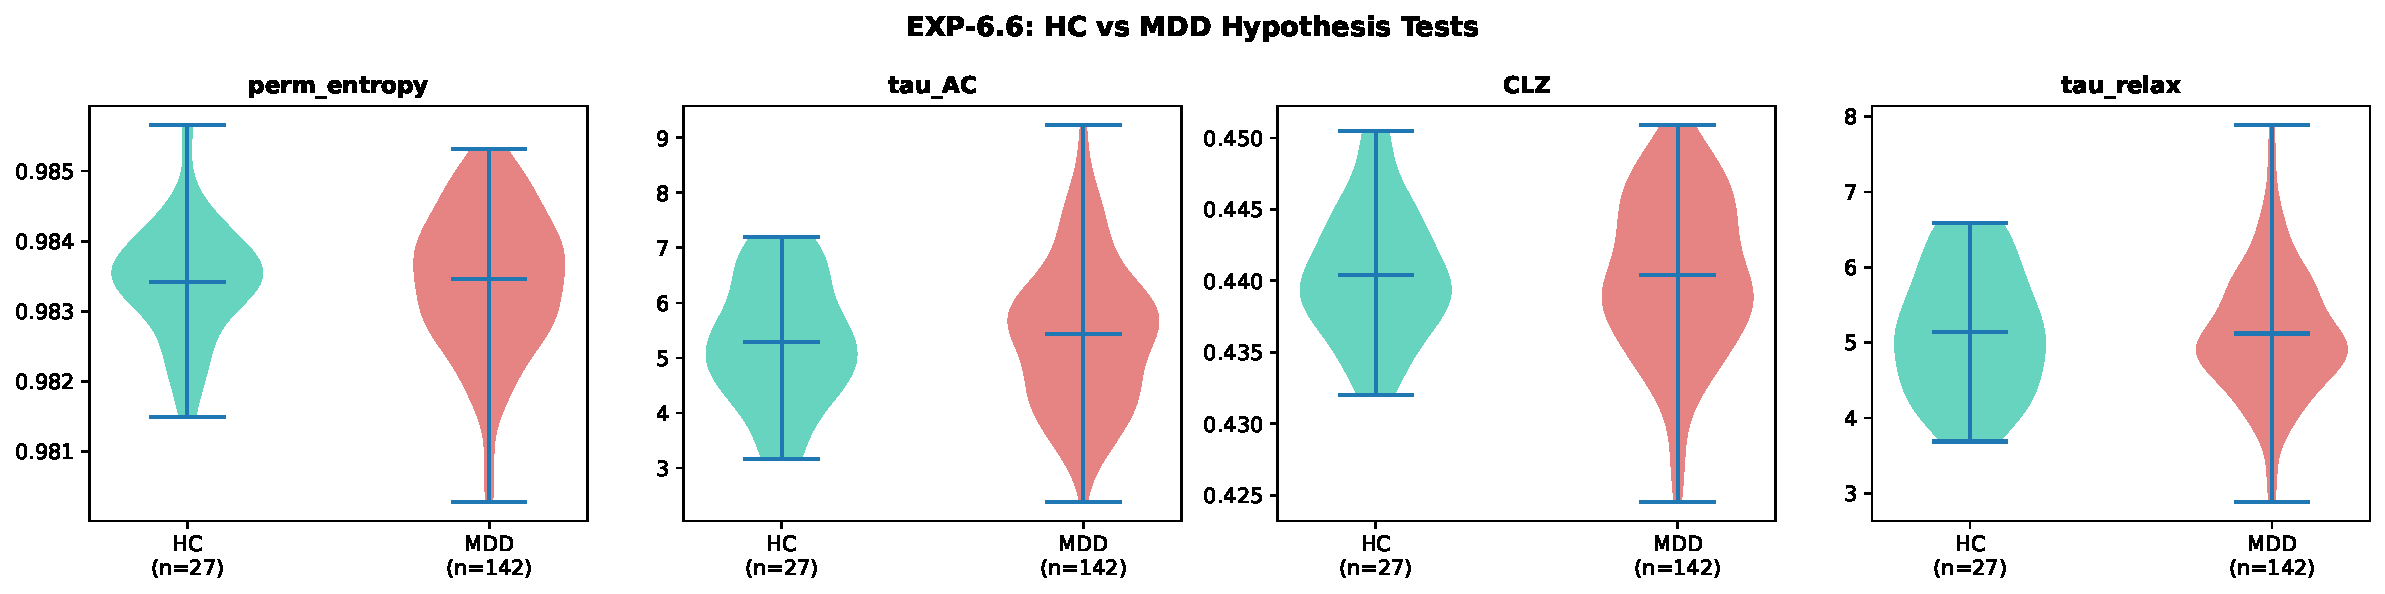
\includegraphics[width=\textwidth]{pictures/chDynamics/fig06_hc_vs_mdd.pdf}
    \caption{Archived HC--MDD screen. The displayed ``HC'' group ($n=27$) includes five participants with incomplete diagnostic panels; the verified complete-case all-negative group has $n=22$. The plotted $\tau_{AC}$ estimate ($d=+0.11$) is therefore descriptive and should be recomputed with the corrected control definition.}
    \label{fig:ch6_hc_vs_mdd}
\end{figure}

The archived point estimates are small ($|d|<0.12$), but the control-definition error and non-significance prevent a directional conclusion. A corrected complete-case analysis must use the 22 verified all-negative participants and report uncertainty without treating a post-hoc detectable-effect calculation as a bound.

\subsection{EXP-6.7: Archived Classifier Results}

The archived three-class classifier using per-channel dynamical features ($238$ dimensions $=34$ channels $\times7$ summaries) has $49.8\%$ balanced accuracy (Figure~\ref{fig:ch6_classification}); the channel-averaged version has $42.2\%$. Adding four auxiliary summaries gives $42.6\%$ in the averaged representation. Because feature and model choices were not evaluated in a fully nested design, these differences are descriptive and do not establish incremental information.

\begin{figure}[H]
    \centering
    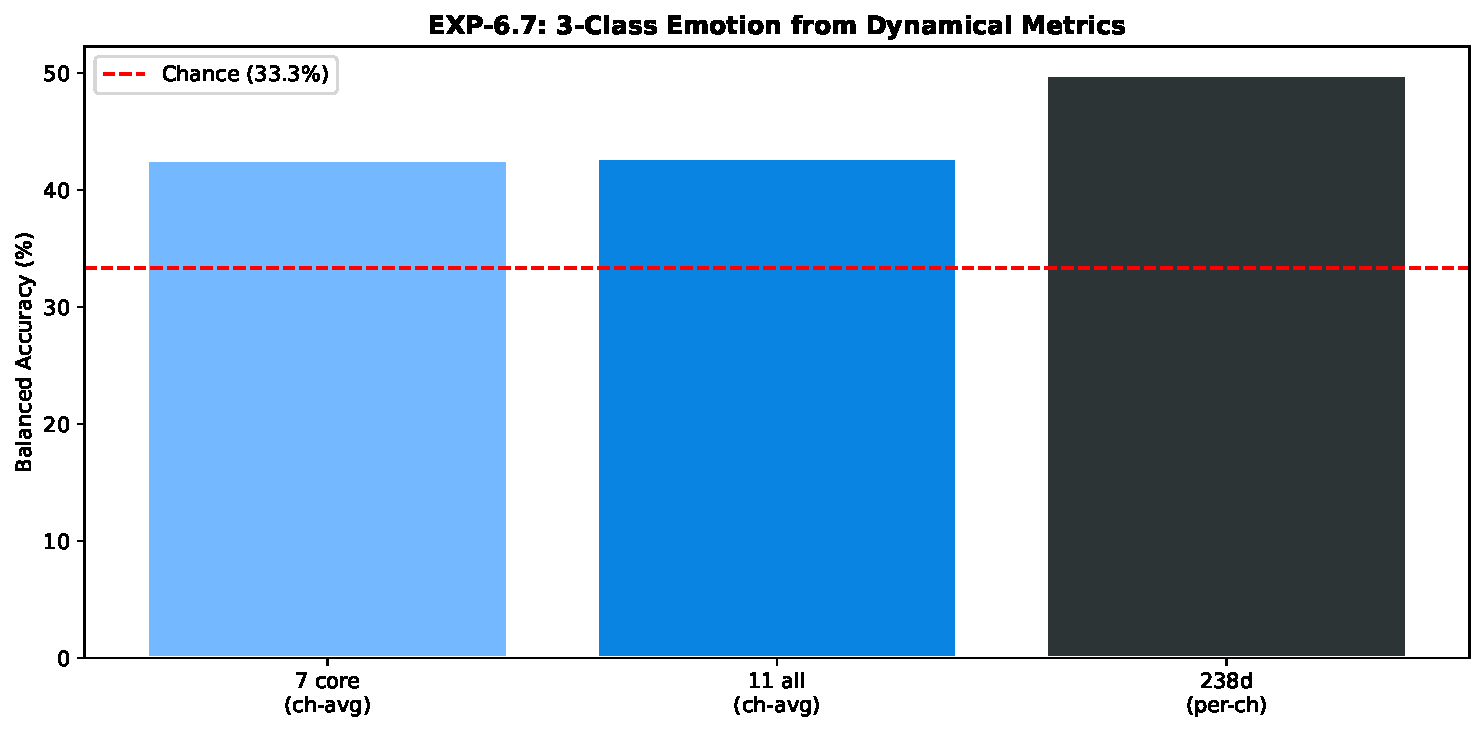
\includegraphics[width=0.75\textwidth]{pictures/chDynamics/fig07_classification.pdf}
    \caption{Archived three-class classification using dynamical summaries. Per-channel features have $49.8\%$ balanced accuracy and channel-averaged features have $42.2\%$. The comparison is descriptive; no nested test establishes the source of the difference.}
    \label{fig:ch6_classification}
\end{figure}

Binary clinical-label estimates using the dynamical summaries are near chance ($49$--$56\%$). The post-hoc maximum for the SUD label is $53.6\%$, which does not establish clinical discrimination. These values provide no basis for claiming that the summaries are clinically sensitive.


\section{Chapter Summary}
\label{sec:dynamics_relationship}

The seven experiments describe the reservoir response using named summaries: total spikes (count), mean firing rate (spikes per neuron per timestep), rate entropy (bits), rate variance, temporal sparsity (fraction of quiescent timesteps), permutation entropy (normalized and dimensionless), and autocorrelation time (timesteps). Their definitions make them inspectable properties of the implemented reservoir response. They are not all physical measurements, and patient-level reliability and clinical actionability are not evaluated.

The findings provide exploratory evidence that these summaries vary with condition. The temporal-structure family has a larger mean absolute Negative--Pleasant effect than the amplitude-tracking family, but the effects are small and the family contrast is descriptive. The archived dynamical-feature classifier reaches $49.8\%$ balanced accuracy. Because model-selection and preprocessing choices were not evaluated in a nested confirmatory design, this value is reported as a descriptive cohort result.

No channel-averaged clinical comparison is detected in EXP-6.3. Per-channel ablation produces near-chance maxima for some diagnoses, but those selected maxima do not establish disorder-specific signals. Chapter~\ref{chap:synthesis} uses the per-channel structure descriptively in the coupling analysis.

Table~\ref{tab:dynamics_relationship_updated} summarizes the relationship between the classification pipeline and the dynamical characterization.

\begin{table}[H]
\centering
\caption{Relationship between the ARSPI-Net classification pipeline and the dynamical characterization.}
\label{tab:dynamics_relationship_updated}
\begin{tabularx}{\textwidth}{>{\raggedright\arraybackslash}p{0.18\textwidth} >{\raggedright\arraybackslash}X >{\raggedright\arraybackslash}X}
\toprule
\textbf{Aspect} & \textbf{Classification (Chapters 3--5)} & \textbf{Dynamical Characterization (This Chapter)} \\
\midrule
Question & Can the system discriminate affective states? & How do reservoir dynamics differ across conditions? \\
Output & Class label $\hat{y}\in\{c_1,\ldots,c_K\}$ & Continuous metric vector $\mathbf{x}\in\mathbb{R}^7$ \\
Condition sensitivity & Archived PCA-dependent estimate; descriptive & Seven nominal Friedman $p<0.05$; exploratory family \\
Clinical sensitivity & Broad exploratory topological search & No detected channel-averaged comparison; near-chance ablation maxima \\
Quantity summarized & Discriminative geometry & Temporal trajectory dynamics \\
\bottomrule
\end{tabularx}
\end{table}


\section{Exploratory Descriptor-to-ERP Alignment}
\label{sec:ch6_erp_alignment}

The seven reservoir summaries have nominal within-cohort condition differences (Section~\ref{sec:ch6_results}). This section reports an exploratory comparison between amplitude-domain analogs and selected ERP scalar summaries. It does not validate a level of explanation fidelity.

Six temporal descriptors were computed from the centered ERP data in the feature window (steps 10--70): mean amplitude (analog of mean firing rate), amplitude variance (analog of spike-count variance), temporal autocorrelation at lag~1 (analog of $\tau_{AC}$), signal complexity (variance of first differences, analog of permutation entropy), peak latency, and temporal asymmetry (early-vs-late energy ratio). The Pearson correlations with classical ERP scalars are:

\begin{table}[H]
\centering
\caption{Exploratory correlations between six amplitude-domain summaries computed in the early feature window and selected ERP scalars. The feature window does not cover the full P300 interval and does not overlap the stated LPP interval, so the correlations are associations rather than component recovery.}
\label{tab:descriptor_erp}
\begin{tabular}{lccc}
\toprule
\textbf{Descriptor} & \textbf{r(P300 amp)} & \textbf{r(LPP amp)} & \textbf{r(P300 lat)} \\
\midrule
Mean amplitude & $+0.647$ & $-0.820$ & $-0.040$ \\
Amplitude variance & $+0.094$ & $-0.069$ & $-0.083$ \\
Temporal autocorrelation & $+0.027$ & $-0.023$ & $-0.133$ \\
Signal complexity & $+0.059$ & $-0.035$ & $+0.046$ \\
Peak latency & $+0.026$ & $-0.018$ & $-0.174$ \\
Temporal asymmetry & $-0.025$ & $+0.022$ & $+0.091$ \\
\bottomrule
\end{tabular}
\end{table}

The early-window mean-amplitude summary has the largest displayed correlations: $r=0.647$ with the P300 scalar and $|r|=0.820$ with the LPP scalar. The largest selected channel correlation is $r=0.837$. Because the early window does not span those components and the strongest channel was selected after inspection, these values are cohort associations and not evidence of component recovery or localization.

The autocorrelation and peak latency descriptors show weak correlations with P300 latency ($r = -0.133$ and $r = -0.174$, respectively). These effect sizes are insufficient for individual-level prediction and provide limited evidence of temporal alignment beyond the mean-amplitude descriptor.

The BSC$_6$ spike-count associations are weaker ($|r|=0.23$ for the LPP scalar and $r=0.33$ for the P300 scalar). The comparison shows that the selected early amplitude summary covaries more strongly with these cohort-level scalars than the selected spike summary; it does not validate clinical explanation fidelity.

NeuCube uses STDP-based connectivity analysis \cite{kasabov_neucube_2014,doborjeh_explainable_2021}; the present summaries instead describe the driven trajectory of a fixed reservoir. For a fixed saved reservoir and input, they are repeatable computational functions. The reported ERP-scalar correlations provide one descriptive comparison, not a validated bridge to physiology and not a head-to-head interpretability evaluation against ProtoPMed-EEG or EEGNet.


\section{Connection to Structure-Function Coupling}
\label{sec:ch6_bridge}

This chapter defines temporal summaries of the driven reservoir. Chapter~\ref{chap:synthesis} compares those summaries with archived graph quantities across the $34$ channel indices using Spearman correlation. The graph quantities inherit the PCA-basis limitations described in Chapter~\ref{chap:arspi_net}; the resulting correlations are descriptive model-to-model associations, not structure--function coupling in the brain.


\section{Summary of Tested Predictions}
\label{sec:dynamics_predictions}

\begin{table}[H]
\centering
\caption{Summary of dynamical predictions and experimental outcomes.}
\label{tab:dynamics_predictions_updated}
\begin{tabularx}{\textwidth}{>{\raggedright\arraybackslash}p{0.20\textwidth} >{\centering\arraybackslash}p{0.10\textwidth} >{\raggedright\arraybackslash}p{0.18\textwidth} >{\raggedright\arraybackslash}X}
\toprule
\textbf{Metric} & \textbf{Symbol} & \textbf{Predicted Direction} & \textbf{Observed Outcome} \\
\midrule
Operation-normalized decoder summary & $\Phi_{dataset}$ & No participant-level direction & Not estimated after fold-safety correction. \\
Lempel--Ziv Complexity & $C_{LZ}$ & $C_{LZ,HC}>C_{LZ,MDD}$ & Effectively zero ($d = +0.004$, $p = 0.57$). \\
Permutation Entropy & $\hat{H}_{\pi}$ & $\hat{H}_{\pi,HC}>\hat{H}_{\pi,MDD}$ & Effectively zero ($d = -0.03$, $p = 0.64$). \\
Relaxation Time & $\tau_{relax}$ & $\tau_{relax,MDD}>\tau_{relax,HC}$ & Opposite direction ($d = -0.02$, $p = 0.56$). \\
Autocorrelation Decay & $\tau_{AC}$ & $\tau_{AC,MDD}>\tau_{AC,HC}$ & Predicted direction ($d = +0.11$, $p = 0.33$). \\
\midrule
\multicolumn{4}{l}{\textit{Exploratory condition comparisons:}} \\
Condition omnibus & all & Condition dependence & Seven nominal Friedman $p<0.05$; no family-level confirmation. \\
Neg vs Pleasant & all & Neg $\neq$ Pleasant & No nominal pairwise result; profiles are similar. \\
\bottomrule
\end{tabularx}
\end{table}

The archived condition screens contain nominal within-participant contrasts. The displayed HC--MDD screen is not a valid complete-case comparison because its $n=27$ control group includes five incomplete diagnostic panels. These analyses therefore cannot establish that condition and person information occupy distinct layers.


\section{Latent Response Organization in the Dynamical Descriptor Space}
\label{sec:ch6_latent_axis}

The final analysis summarizes the $7$-metric by $34$-channel descriptor matrix with PCA and exploratory clustering. It asks how much in-sample variation lies along the leading components and whether the fitted scores are associated with condition or diagnostic metadata.

\subsection{Methods}

Subject-level descriptor vectors were constructed by averaging the seven dynamical metrics across the three conditions for each of the $211$ subjects, yielding a $211\times238$ matrix. Featurewise means and standard deviations were estimated from that subject-averaged matrix, and PCA was fit to the standardized matrix. Condition-specific vectors were standardized with those same featurewise parameters and projected onto the in-sample PC1 loading. The resulting condition test is descriptive of this cohort; PC1 was not learned in an independent sample. Friedman and Bonferroni-corrected Wilcoxon tests assess repeated condition scores. Clinical associations use Mann--Whitney $U$. A median split and several clustering methods are secondary descriptive analyses. Cluster quality is evaluated by silhouette, Davies--Bouldin, and Calinski--Harabasz indices; repeated initializations assess only algorithmic stability, not biological or test--retest reliability.

\subsection{Principal Component Analysis of the Descriptor Space}

In the fitted sample, PC1 explains $19.1\%$ of descriptor variance, while PC2 and PC3 explain $11.5\%$ and $7.7\%$, respectively. The first three components account for $38.3\%$ in total, and $54$ components are needed to reach $90\%$.

PCA signs are arbitrary. For consistency with the condition-score figure, the axis is oriented so that negative scores correspond to higher excitability: mean firing rate ($-0.073$), rate entropy ($-0.085$), permutation entropy ($-0.070$), and active ratio ($-0.078$) point toward that end, while autocorrelation time ($+0.055$) points toward persistence. The label \textbf{excitability--persistence axis} is a descriptive interpretation of these small, channel-distributed loadings rather than a physiological measurement.

\begin{figure}[t]
    \centering
    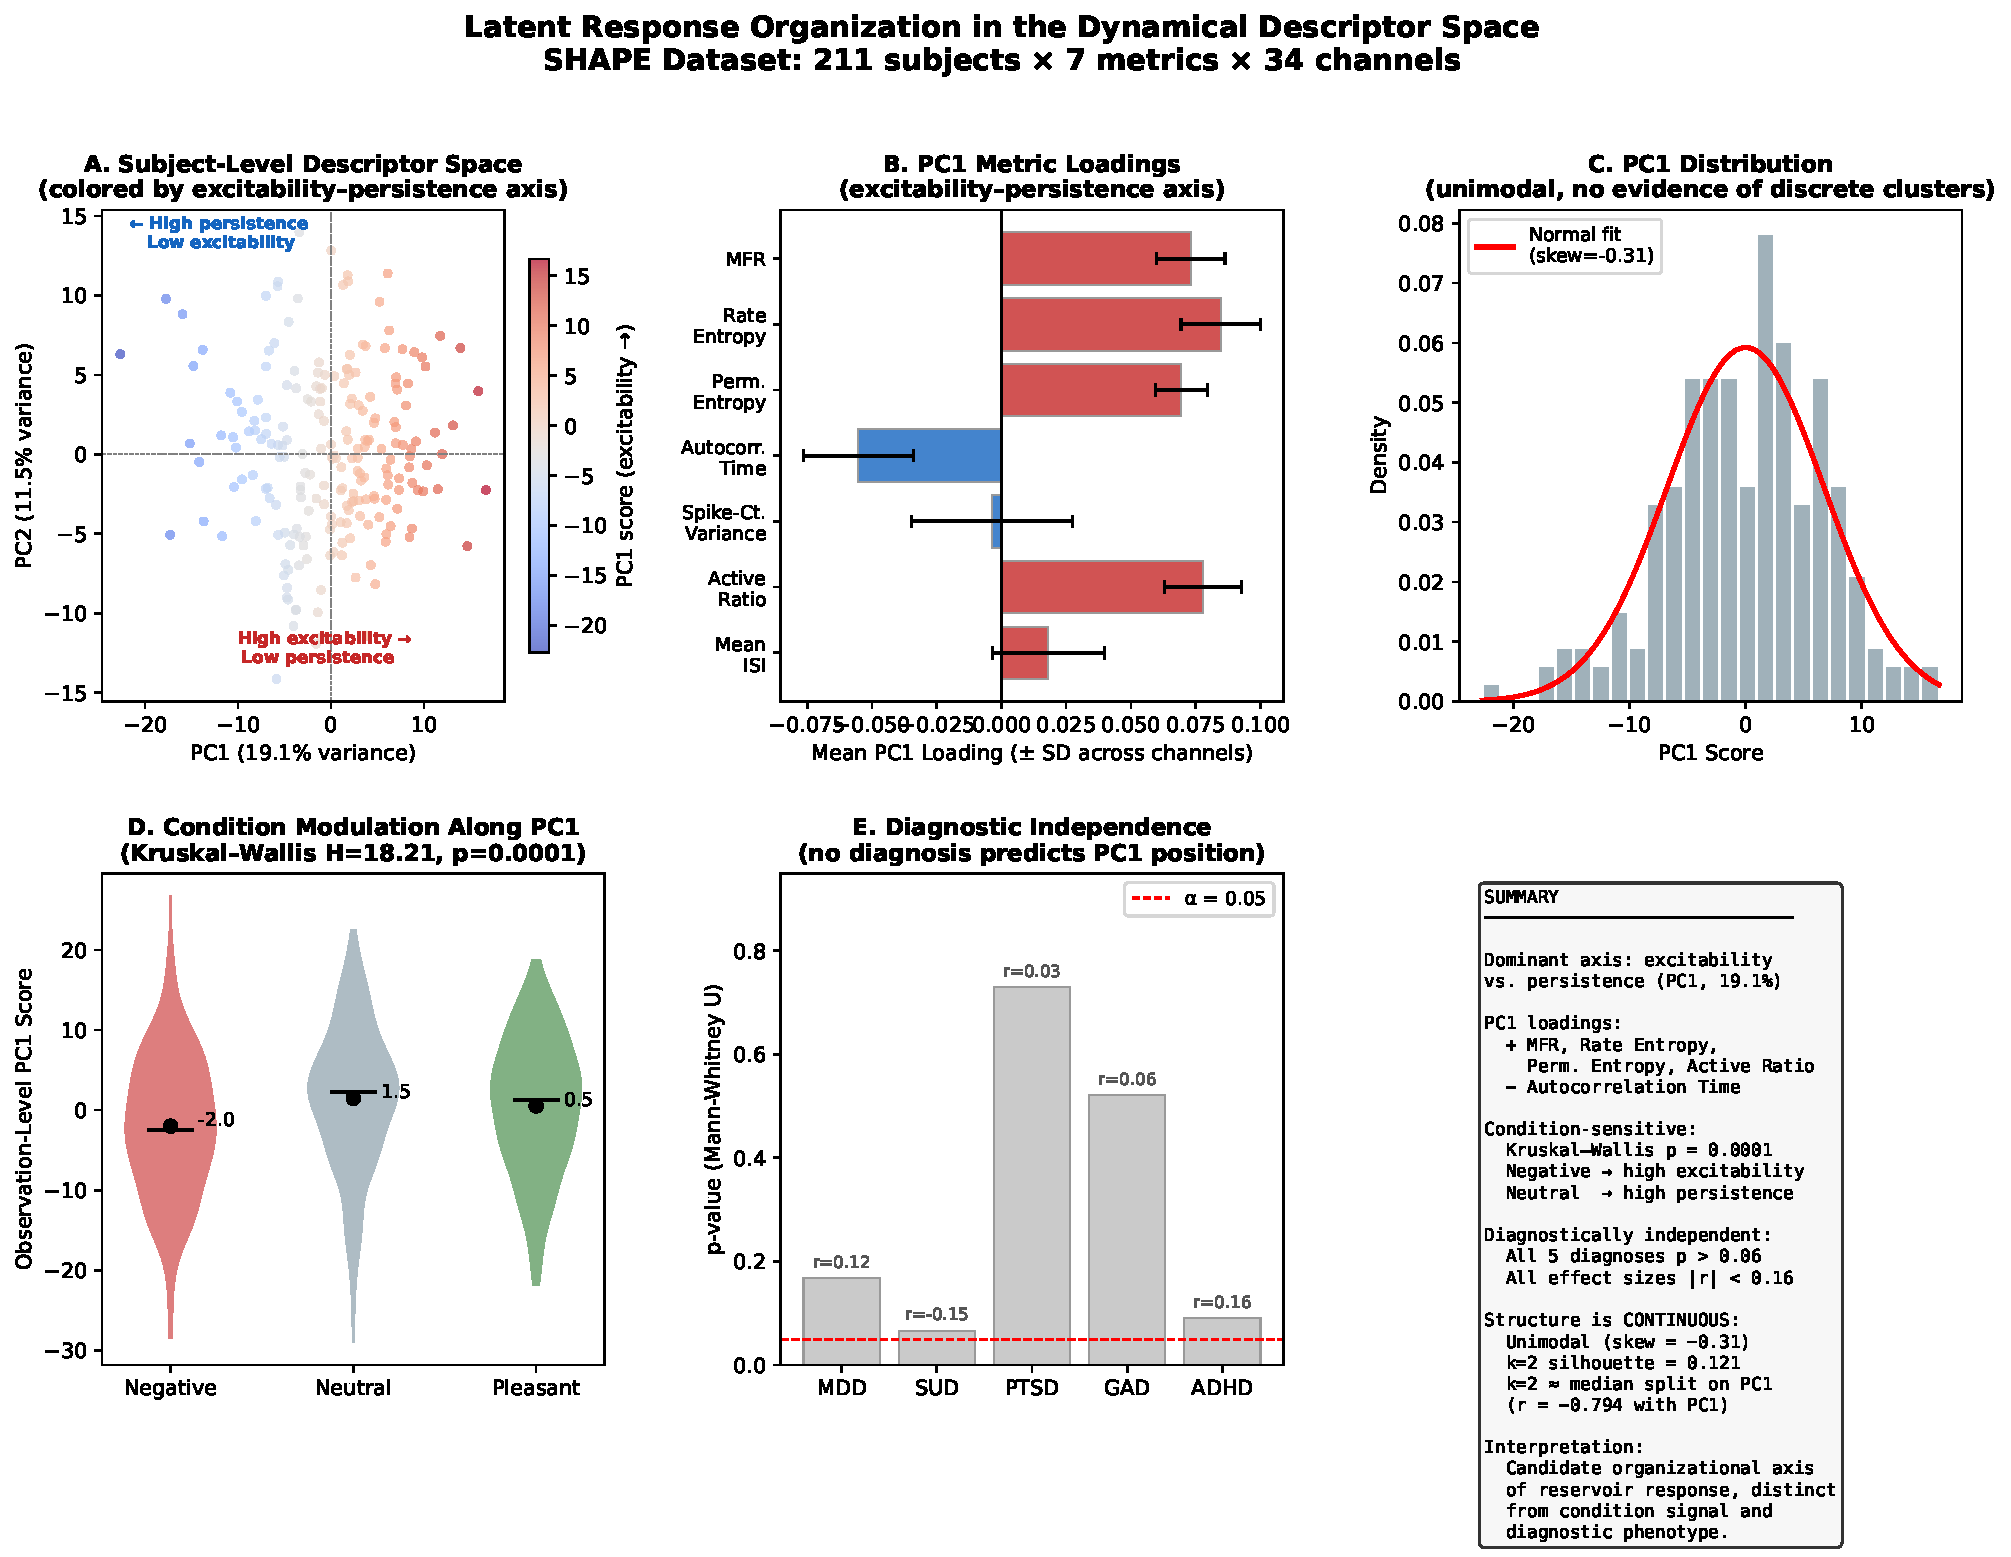
\includegraphics[width=\textwidth]{pictures/chDynamics/fig_latent_axis.pdf}
    \caption{Descriptive organization of the dynamical-summary space. PC1 explains $19.1\%$ of in-sample variance and is labeled excitability--persistence from its small distributed loadings. The condition effect is small ($W=0.057$), the ADHD median-split association is uncorrected, and the one-component BIC preference does not prove a continuous population structure.}
    \label{fig:latent_axis}
\end{figure}

\subsection{Condition Modulation Along the Latent Axis}

To test condition modulation with the correct repeated-measures design, each subject's three condition-specific descriptor vectors were projected onto the PC1 loading vector learned from the subject-level PCA (as described in the Methods), producing three repeated PC1-aligned scores per subject. The Friedman test is the appropriate non-parametric repeated-measures test for this design.

Scores along the in-sample PC1 loading differ by condition (Friedman $\chi^2=24.00$, $p=6\times10^{-6}$, Kendall's $W=0.057$). The oriented means are $-2.00$ for Negative, $+1.47$ for Neutral, and $+0.53$ for Pleasant. Bonferroni-adjusted pairwise tests give small $p$ values for Negative versus the other two conditions and $p=0.29$ for Neutral versus Pleasant. The effect size is small, and because the axis was learned from the same cohort, the result requires out-of-sample confirmation.

\subsection{Association with Psychiatric Diagnosis}

None of the five continuous PC1 group comparisons meets the Bonferroni-adjusted threshold: MDD ($p = 0.17$, $r_{pb} = -0.12$), SUD ($p = 0.07$, $r_{pb} = 0.14$), PTSD ($p = 0.73$, $r_{pb} = -0.01$), GAD ($p = 0.52$, $r_{pb} = -0.04$), and ADHD ($p = 0.09$, $r_{pb} = -0.13$). The sample effect sizes satisfy $|r_{pb}| \leq 0.14$; the adjusted threshold across these five tests is $\alpha_{adj}=0.01$.

As a secondary check, PC1 was split at its sample median and tested against each diagnosis with $\chi^2$ contingency analysis. Four comparisons have Cram\'{e}r's $V<0.08$. ADHD has uncorrected $\chi^2=4.10$, $p=0.043$, and Cram\'{e}r's $V=0.14$, but does not meet the five-test adjusted threshold. Because dichotomization was secondary and loses information, this result is not evidence of an ADHD subgroup. PC1 remains an in-sample description of the descriptor matrix.

\subsection{Discretization and Cluster Structure}

Clustering was evaluated for $k=2$ through $k=6$. The largest silhouette score is only $0.121$ at $k=2$; Gaussian-mixture and spectral variants yield similarly weak separation. The $k=2$ result is seed-stable for the tested initializations (ARI $=1.00$) and strongly associated with PC1 ($r=-0.794$). This is algorithmic consistency in the same data, not biological reliability, and the weak silhouette does not support discrete subpopulations.

A one-component Gaussian mixture has lower BIC than a two-component model ($\Delta\text{BIC}=-14.5$ in favor of one). Together with the weak silhouette, this provides no evidence for a natural two-group boundary. It does not prove that the population distribution is continuous or that the tentative axis has physiological meaning.

\subsection{Summary}

PC1 explains $19.1\%$ of the in-sample descriptor variance and has a small condition association ($W=0.057$). Continuous diagnosis associations are small, and the uncorrected ADHD median-split result does not survive adjustment. BIC favors one component and the $k=2$ silhouette is weak ($0.121$), so the data provide no clear evidence of discrete groups. The ``excitability--persistence'' label is a tentative description of loadings and requires out-of-sample and test--retest evaluation.
